%!TEX root = ../template.tex
%%%%%%%%%%%%%%%%%%%%%%%%%%%%%%%%%%%%%%%%%%%%%%%%%%%%%%%%%%%%%%%%%%%%
%% appendix7.tex
%% NOVA thesis document file
%%
%% Chapter with Simulation Test Results
%%%%%%%%%%%%%%%%%%%%%%%%%%%%%%%%%%%%%%%%%%%%%%%%%%%%%%%%%%%%%%%%%%%%
\chapter{Simulation Test Results}
\label{app:simulation_test_results}

\section{Camera Spatial Data Processing}
\label{sec:simulation_test_results_appendix_camera_spatial_data}

\begin{figure}[htbp]
	\centering
	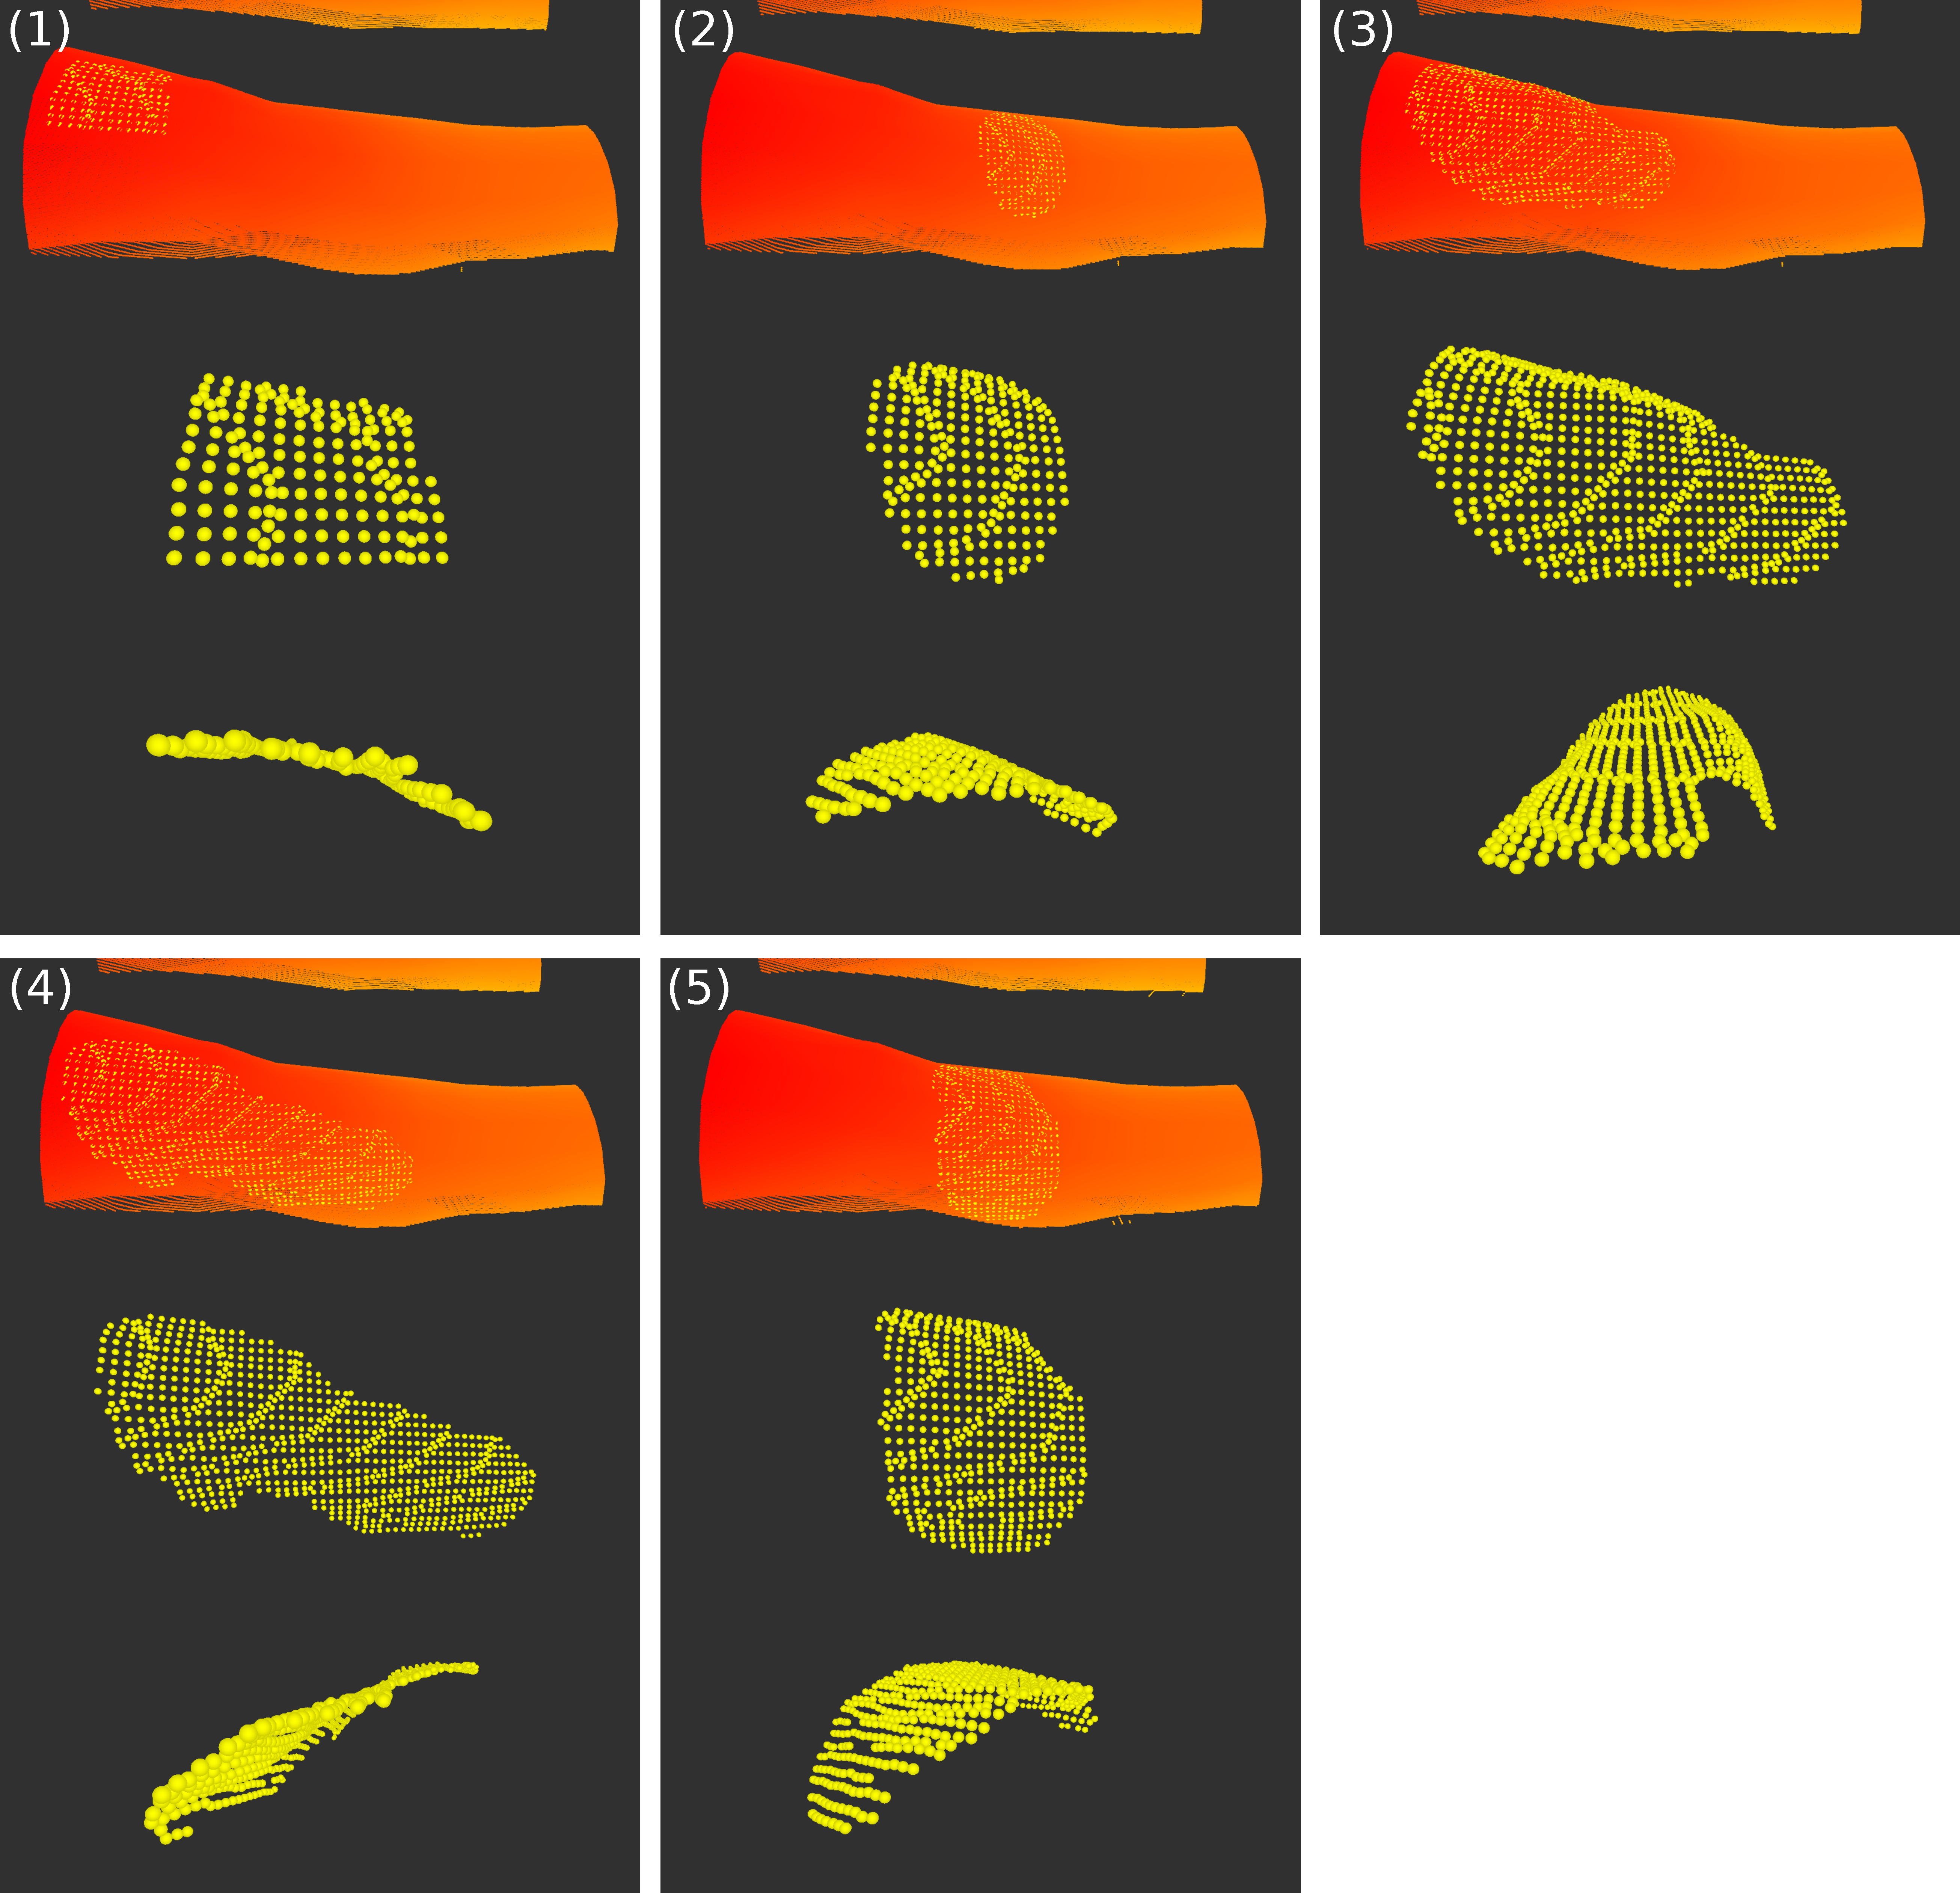
\includegraphics[width=.72\textwidth]{simulation_test_results_appendix_camera_spatial_data_pcloud}
	\caption{Wound model's point cloud. Each wound model has three representations of the associated point cloud. (top) Wound point cloud in yellow superimposed on the patient model's leg point cloud. (middle) Centred zoom on the wound point cloud. The perspective is the same as top. (bottom) Different perspective of the point cloud to evidence its non-planar nature. }
	\label{fig:simulation_test_results_appendix_camera_spatial_data_pcloud}
\end{figure}

% section simulation_test_results_appendix_camera_spatial_data

\section{Path Planning}
\label{sec:simulation_test_results_appendix_path_planning}

\begin{figure}[htbp]
	\centering
	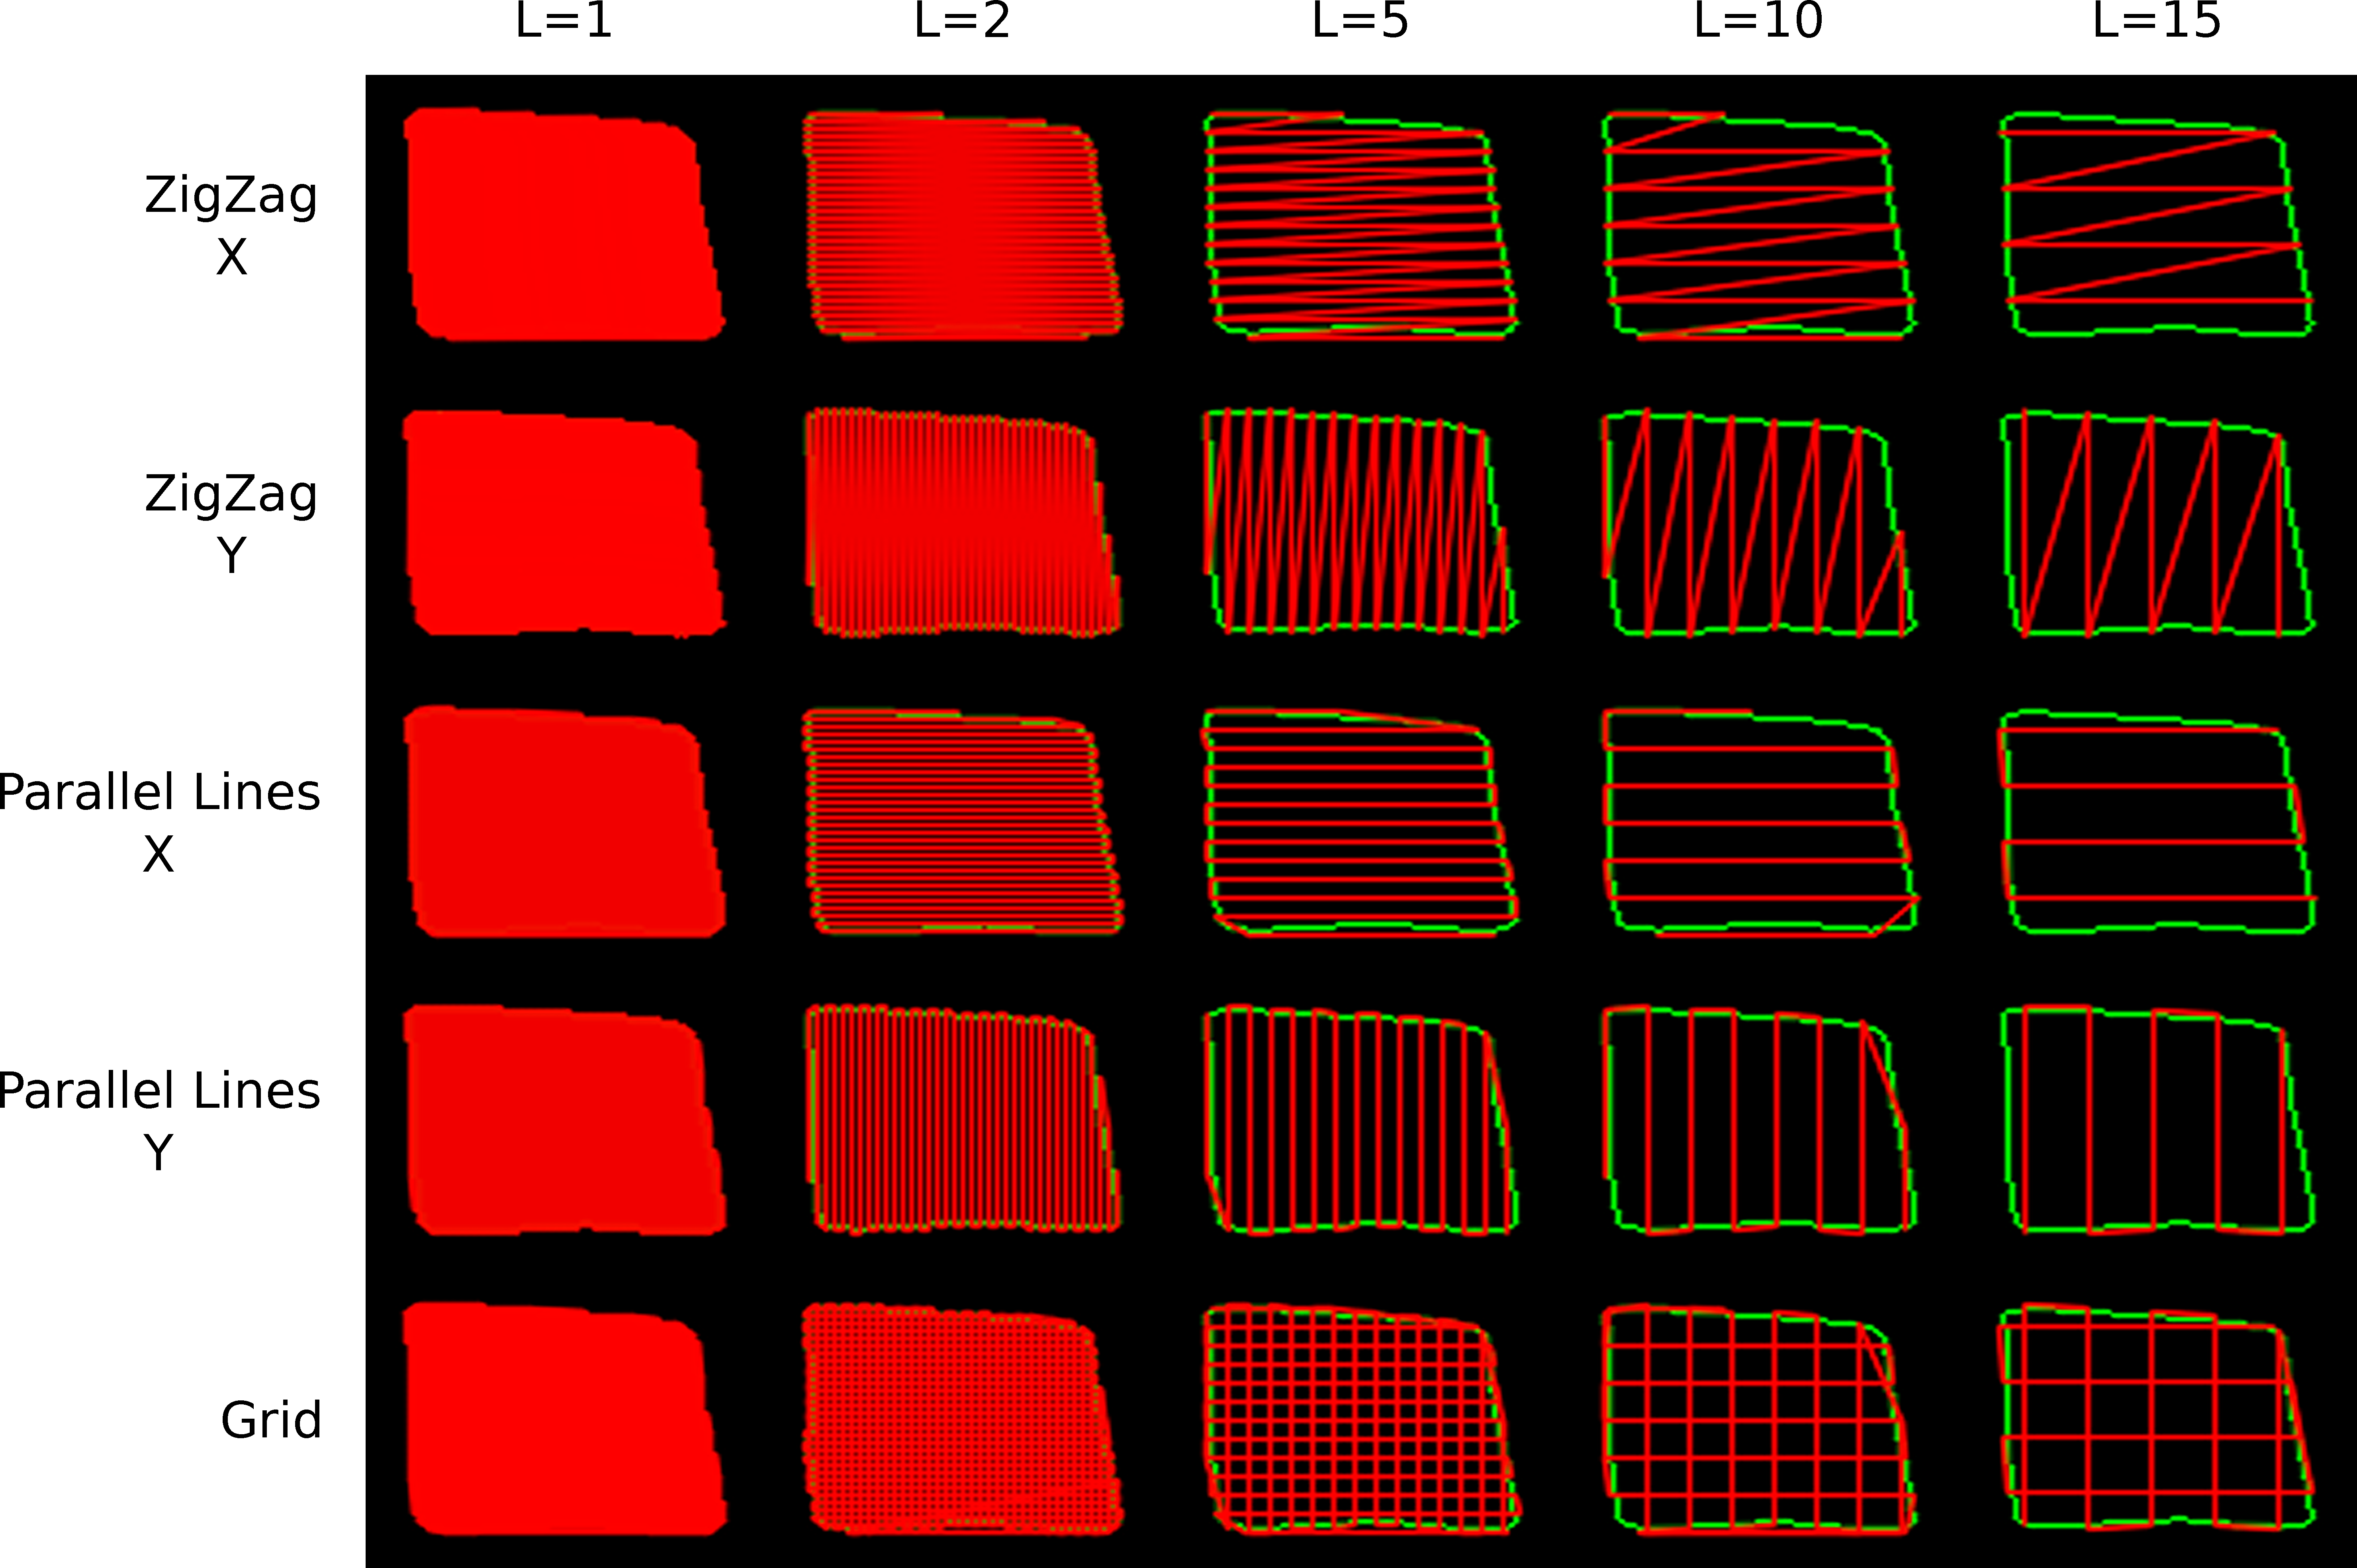
\includegraphics[width=.85\textwidth]{simulation_test_results_appendix_toolpath_wound_1}
	\caption{Path planning for wound model 1. The green line represents the segmented wound contour. The red line is the planned path. From left to right, the distance between lines, $L$, in pixels, is increasing. Smaller $L$ means more wound filling but also more bioink consumption. From top top bottom, the different paths are displayed. Each line corresponds to a different path planning strategy.}
	\label{fig:simulation_test_results_appendix_toolpath_wound_1}
\end{figure}

\begin{figure}[htbp]
	\centering
	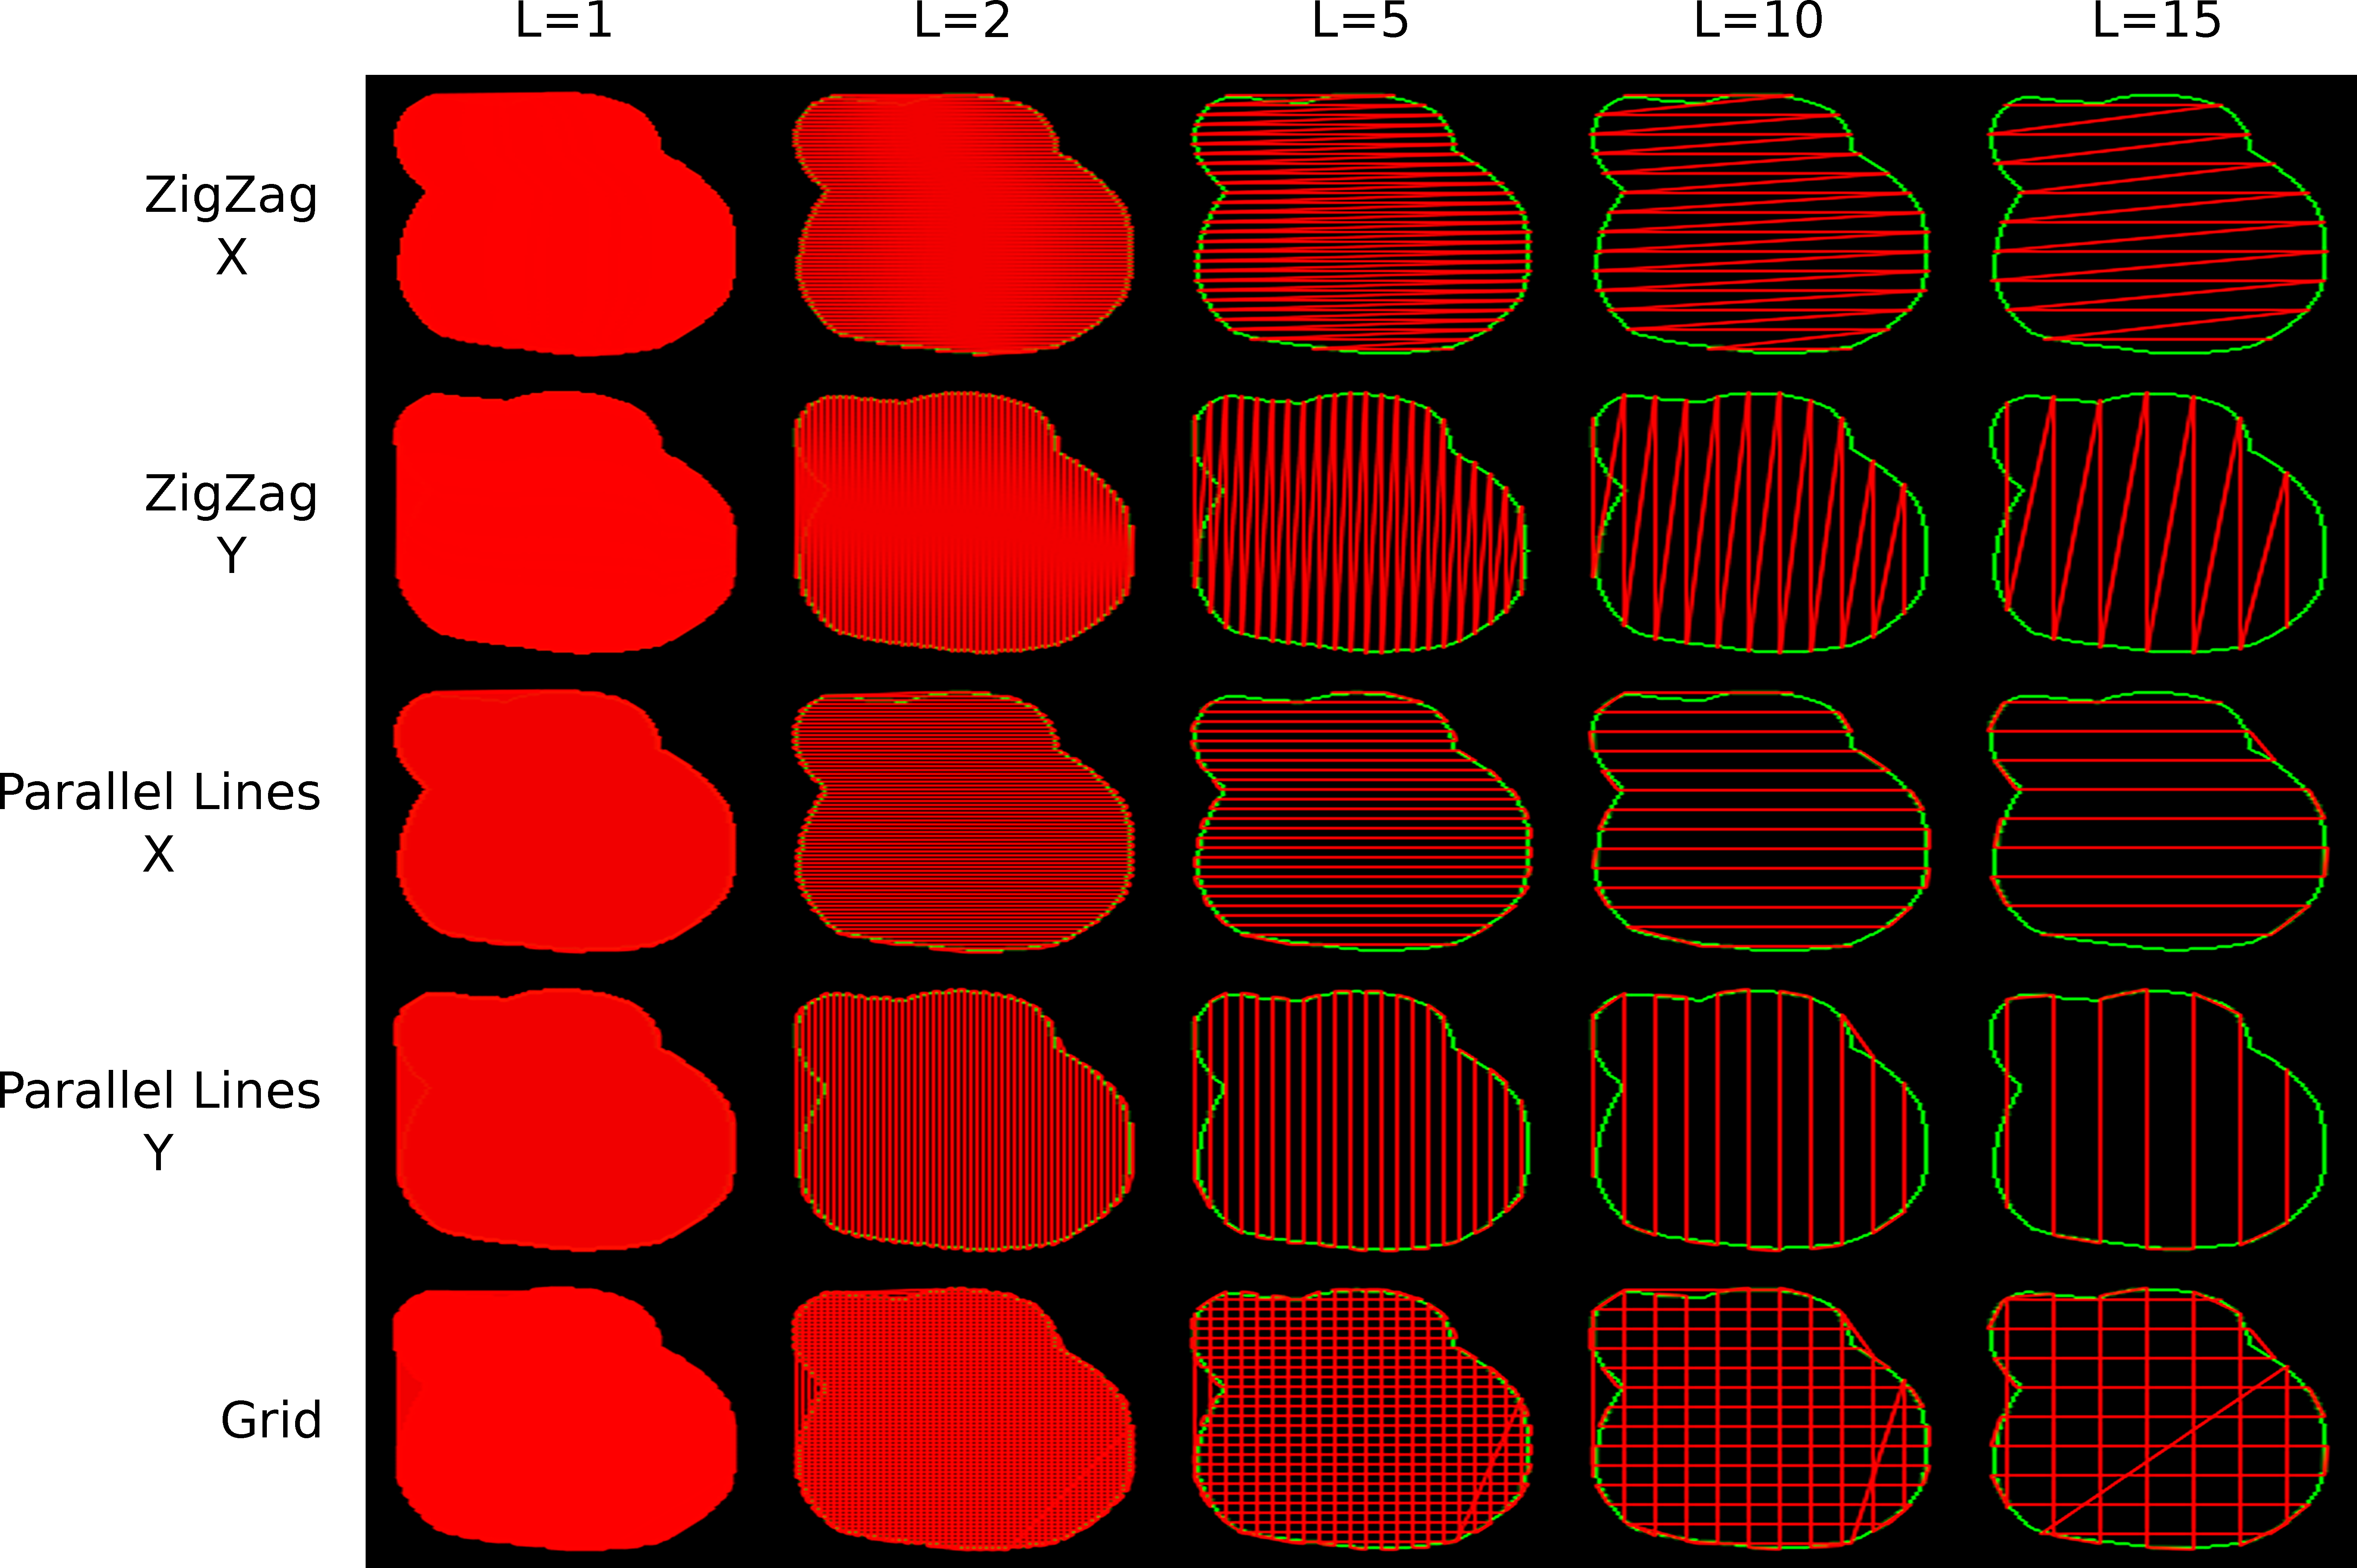
\includegraphics[width=.85\textwidth]{simulation_test_results_appendix_toolpath_wound_2}
	\caption{Path planning for wound model 2. The green line represents the segmented wound contour. The red line is the planned path. From left to right, the distance between lines, $L$, in pixels, is increasing. Smaller $L$ means more wound filling but also more bioink consumption. From top top bottom, the different paths are displayed. Each line corresponds to a different path planning strategy.}
	\label{fig:simulation_test_results_appendix_toolpath_wound_2}
\end{figure}

\begin{figure}[htbp]
	\centering
	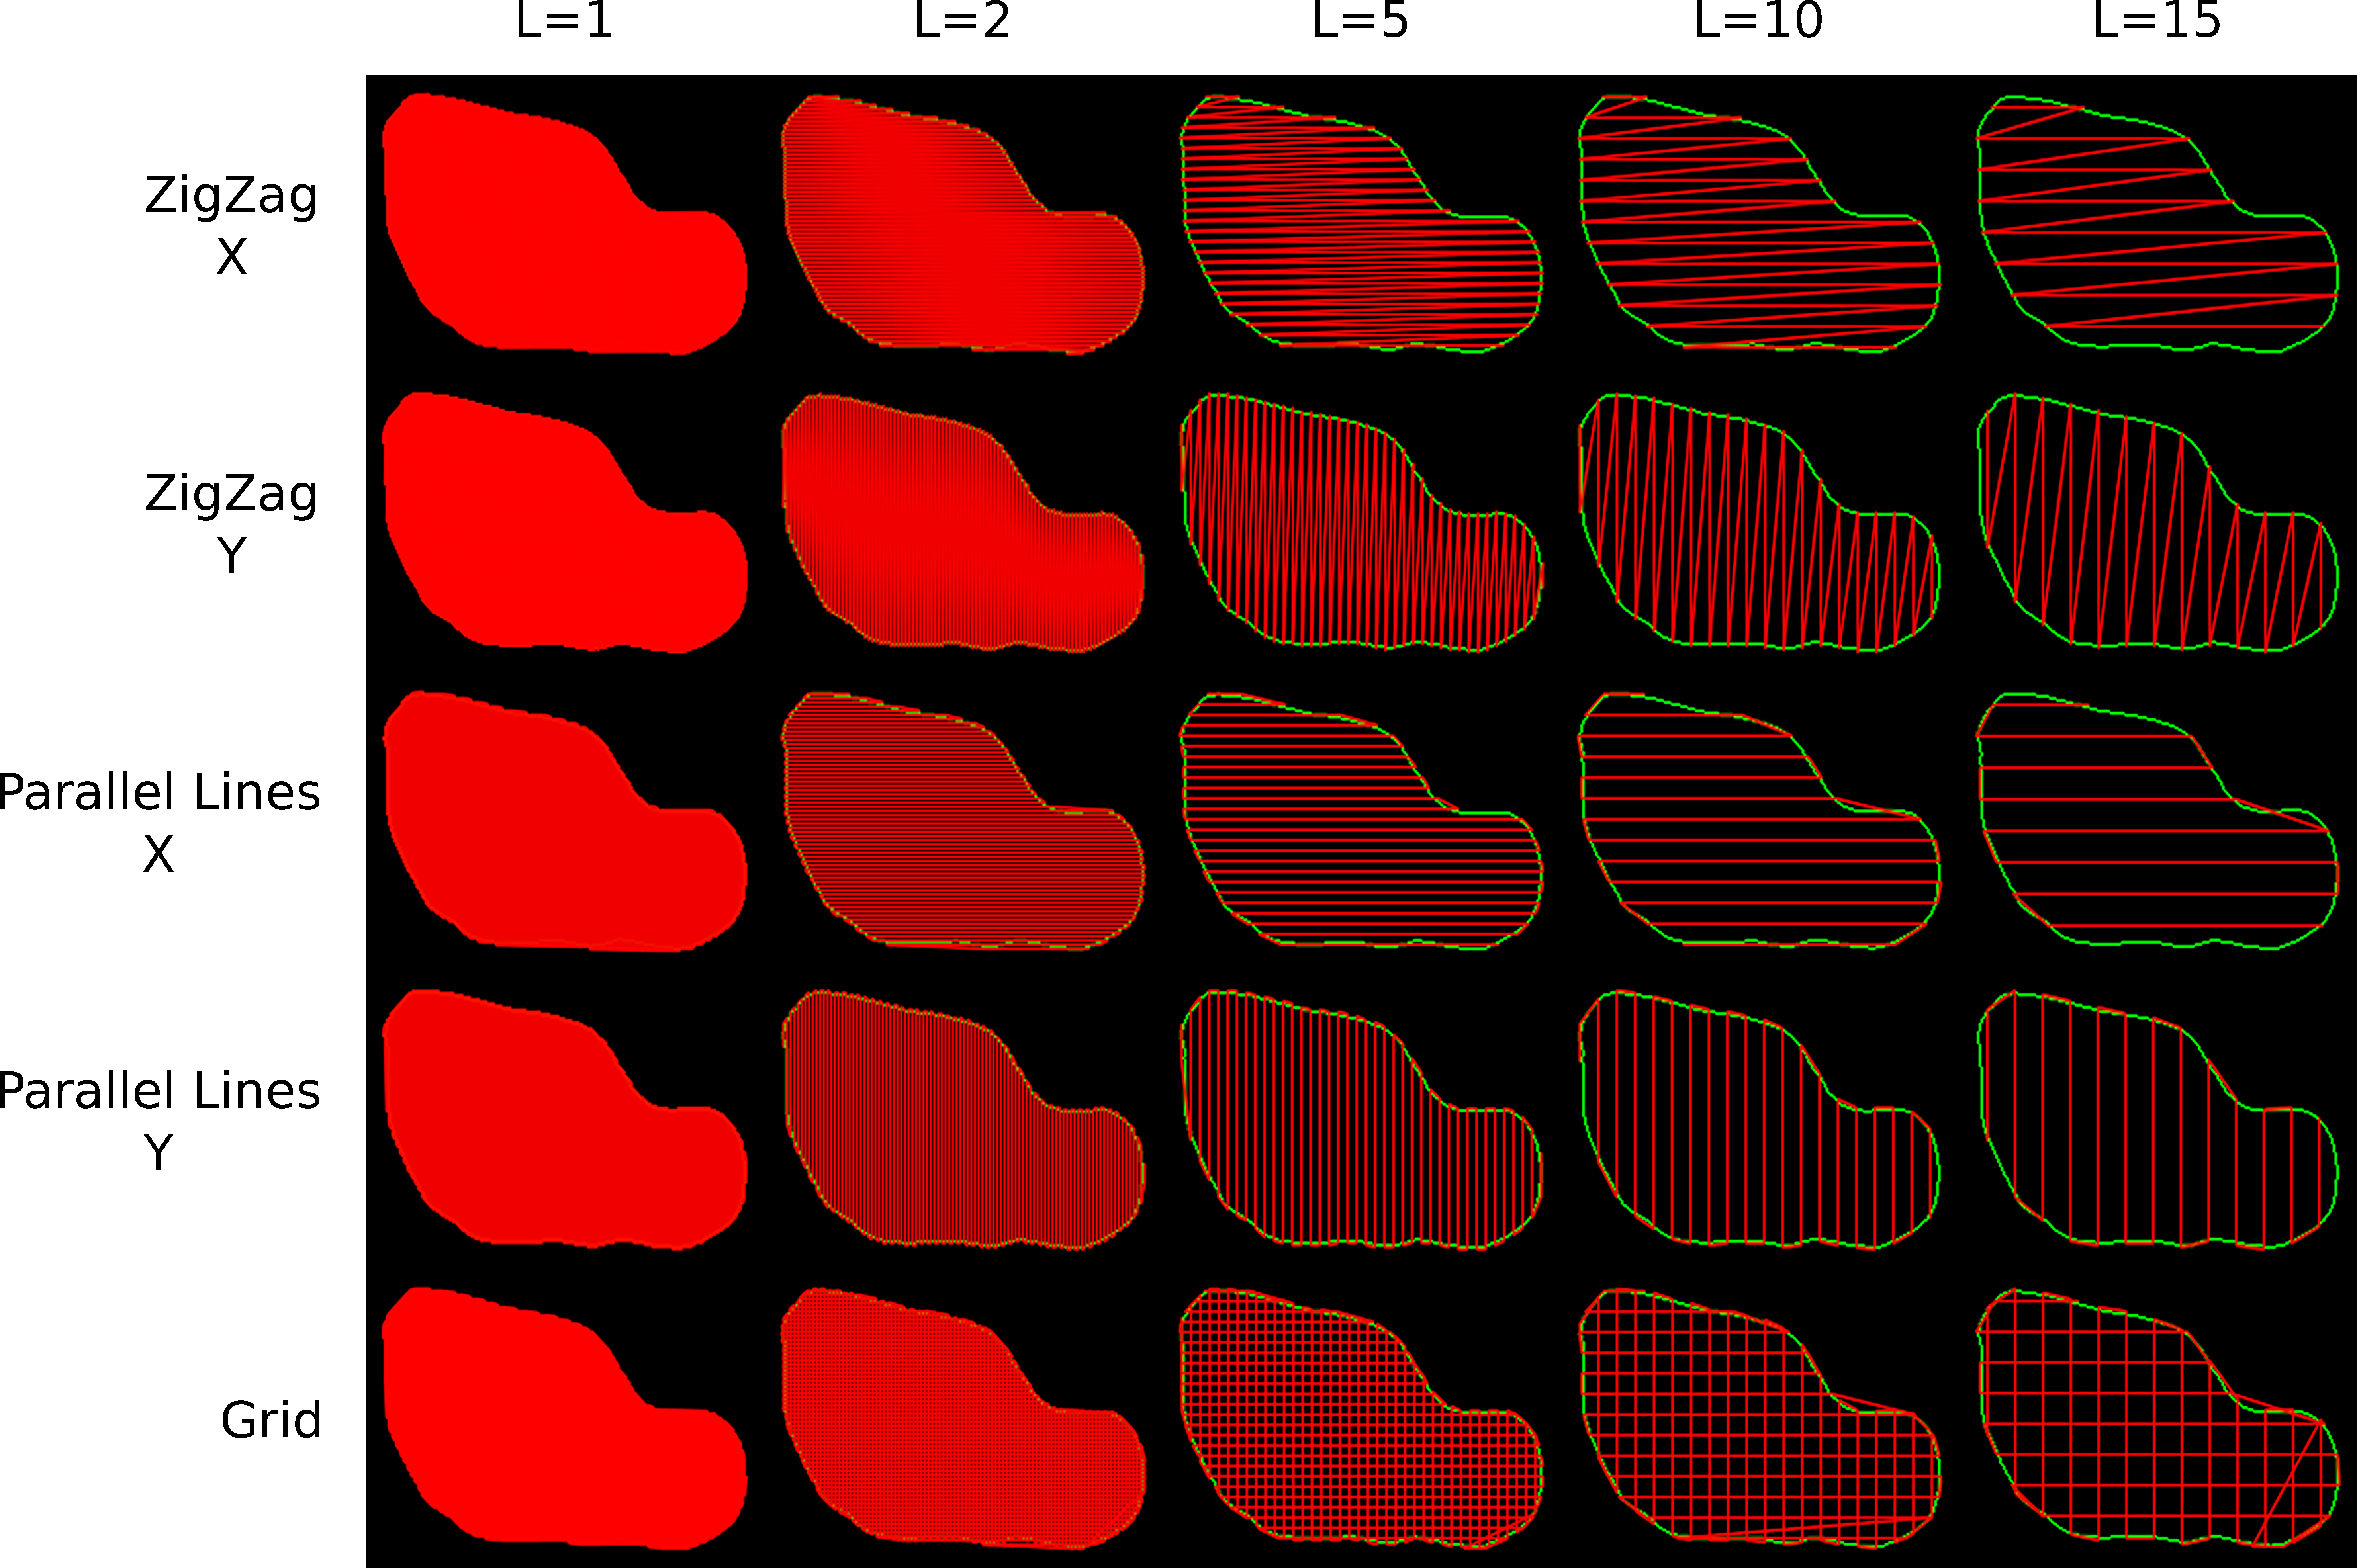
\includegraphics[width=.85\textwidth]{simulation_test_results_appendix_toolpath_wound_3}
	\caption{Path planning for wound model 3. The green line represents the segmented wound contour. The red line is the planned path. From left to right, the distance between lines, $L$, in pixels, is increasing. Smaller $L$ means more wound filling but also more bioink consumption. From top top bottom, the different paths are displayed. Each line corresponds to a different path planning strategy.}
	\label{fig:simulation_test_results_appendix_toolpath_wound_3}
\end{figure}

\begin{figure}[htbp]
	\centering
	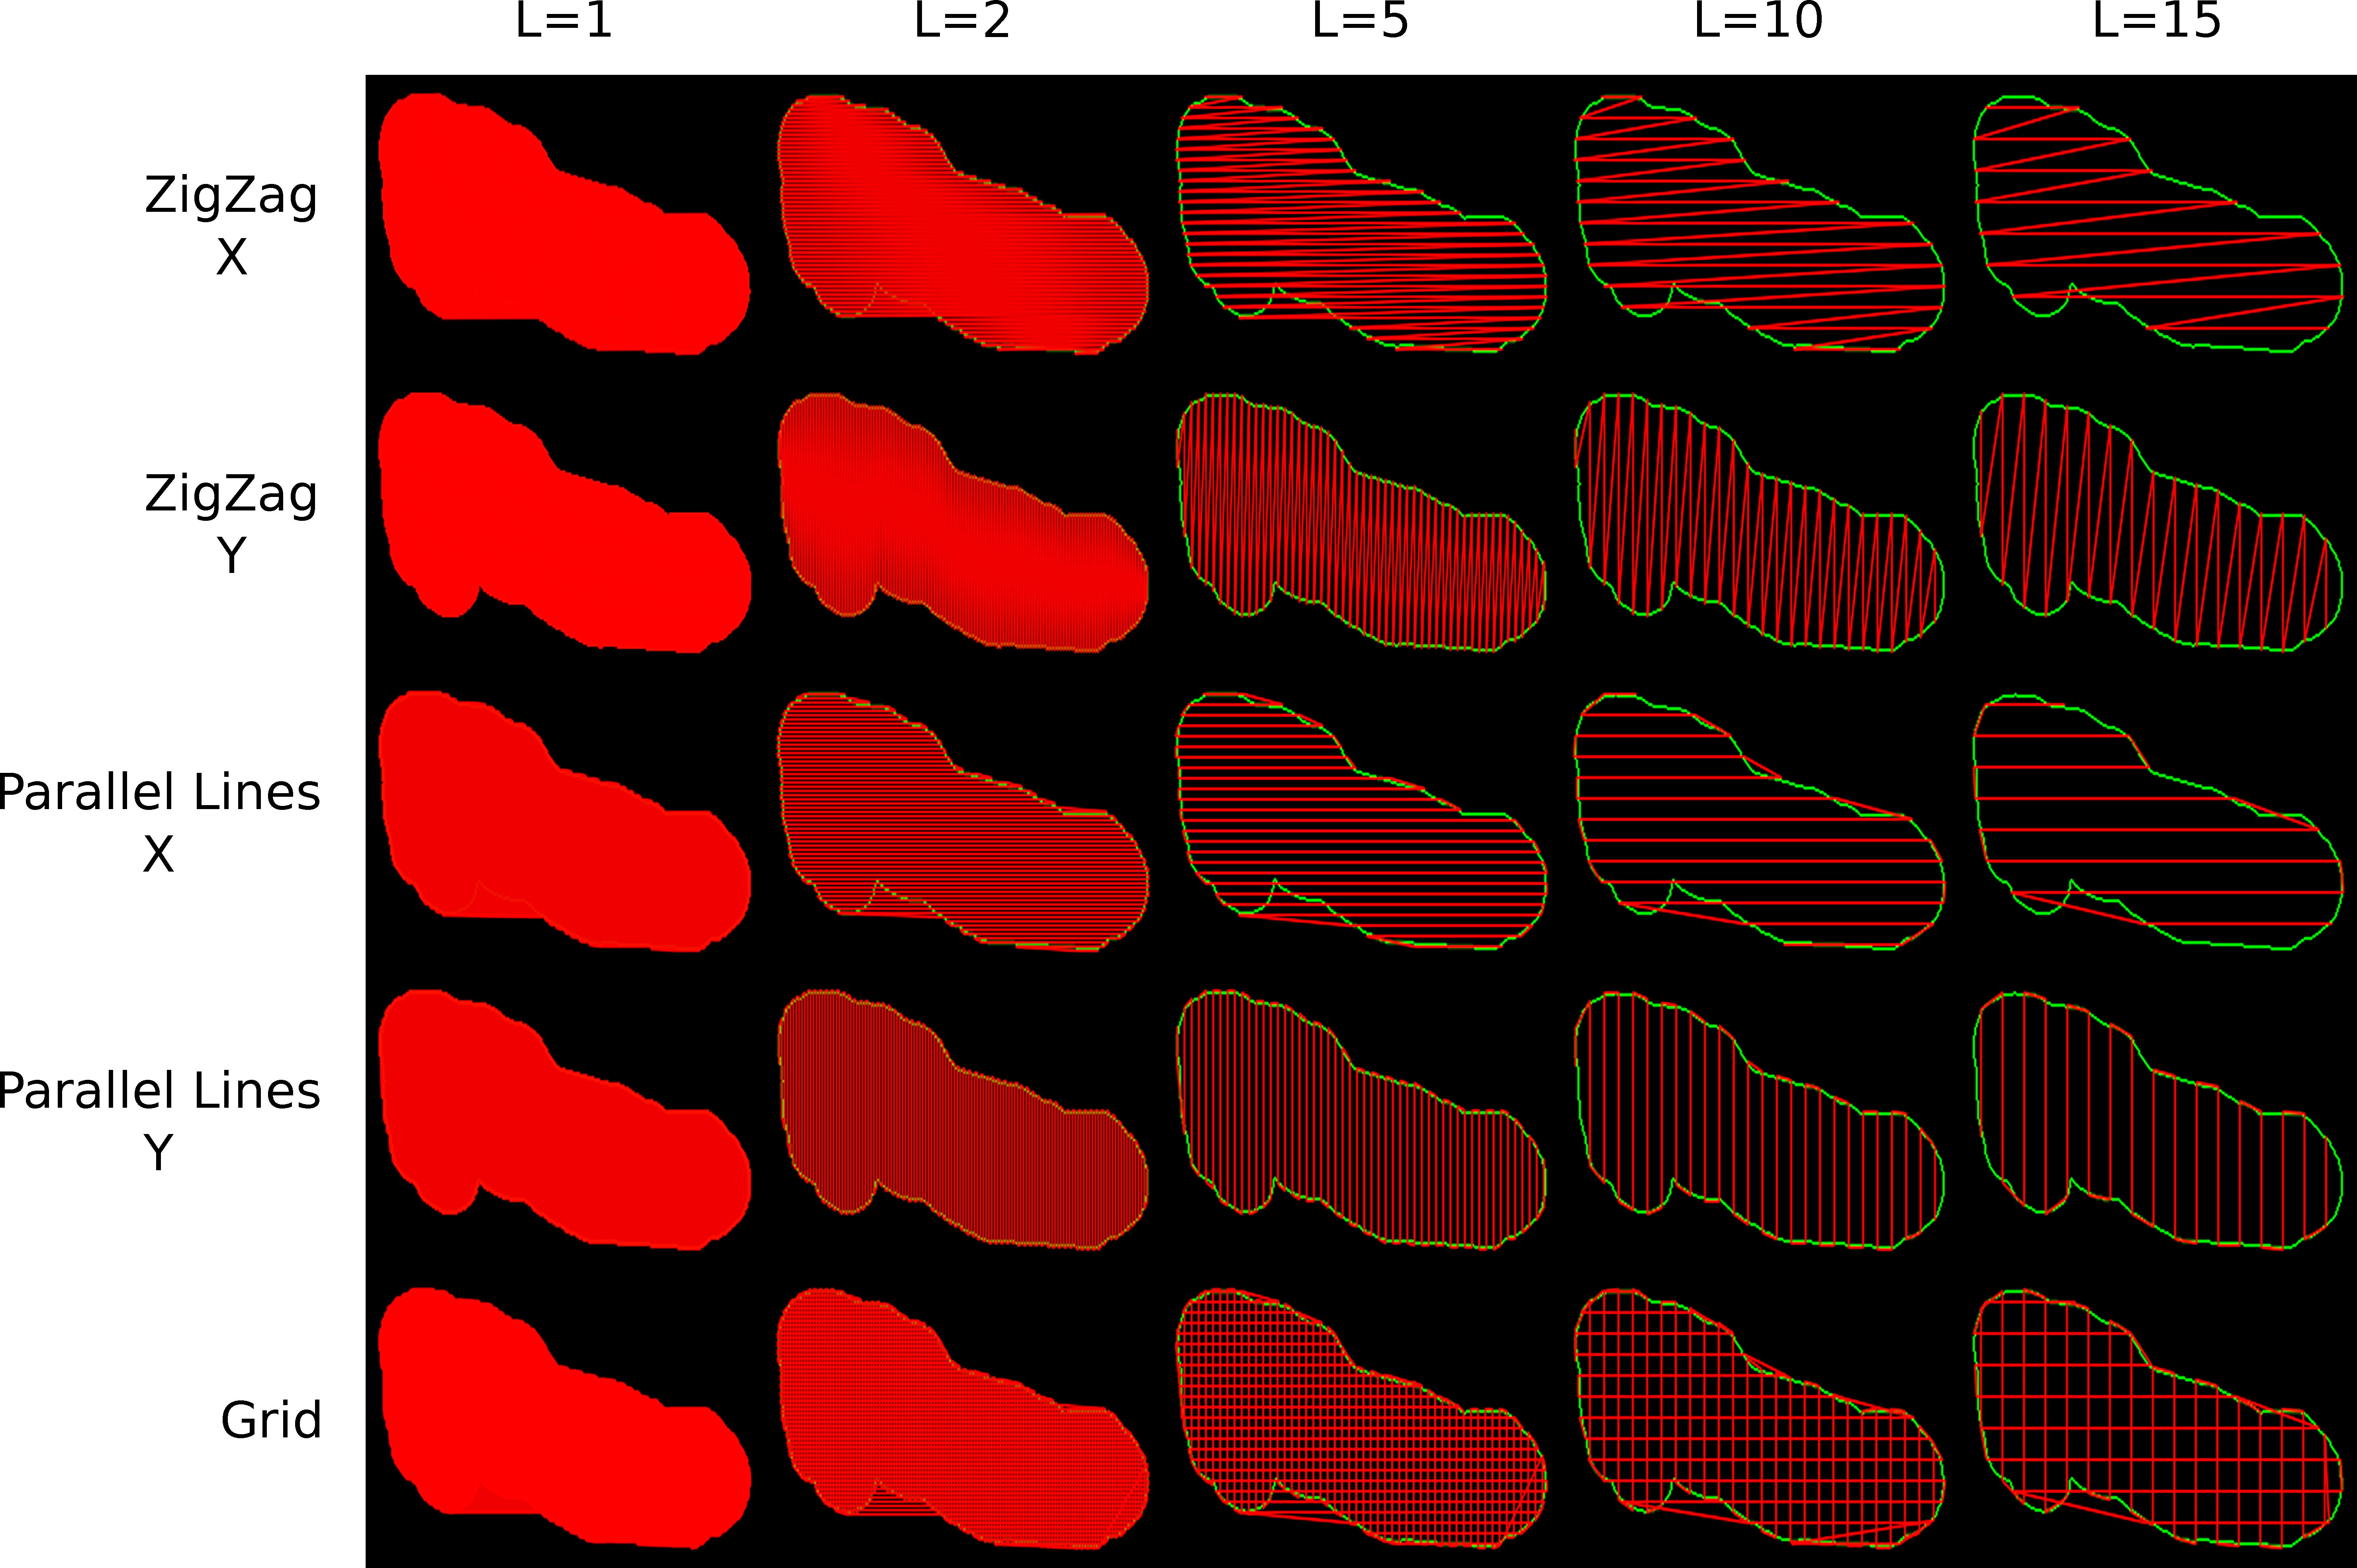
\includegraphics[width=.85\textwidth]{simulation_test_results_appendix_toolpath_wound_4}
	\caption{Path planning for wound model 4. The green line represents the segmented wound contour. The red line is the planned path. From left to right, the distance between lines, $L$, in pixels, is increasing. Smaller $L$ means more wound filling but also more bioink consumption. From top top bottom, the different paths are displayed. Each line corresponds to a different path planning strategy.}
	\label{fig:simulation_test_results_appendix_toolpath_wound_4}
\end{figure}

\begin{figure}[htbp]
	\centering
	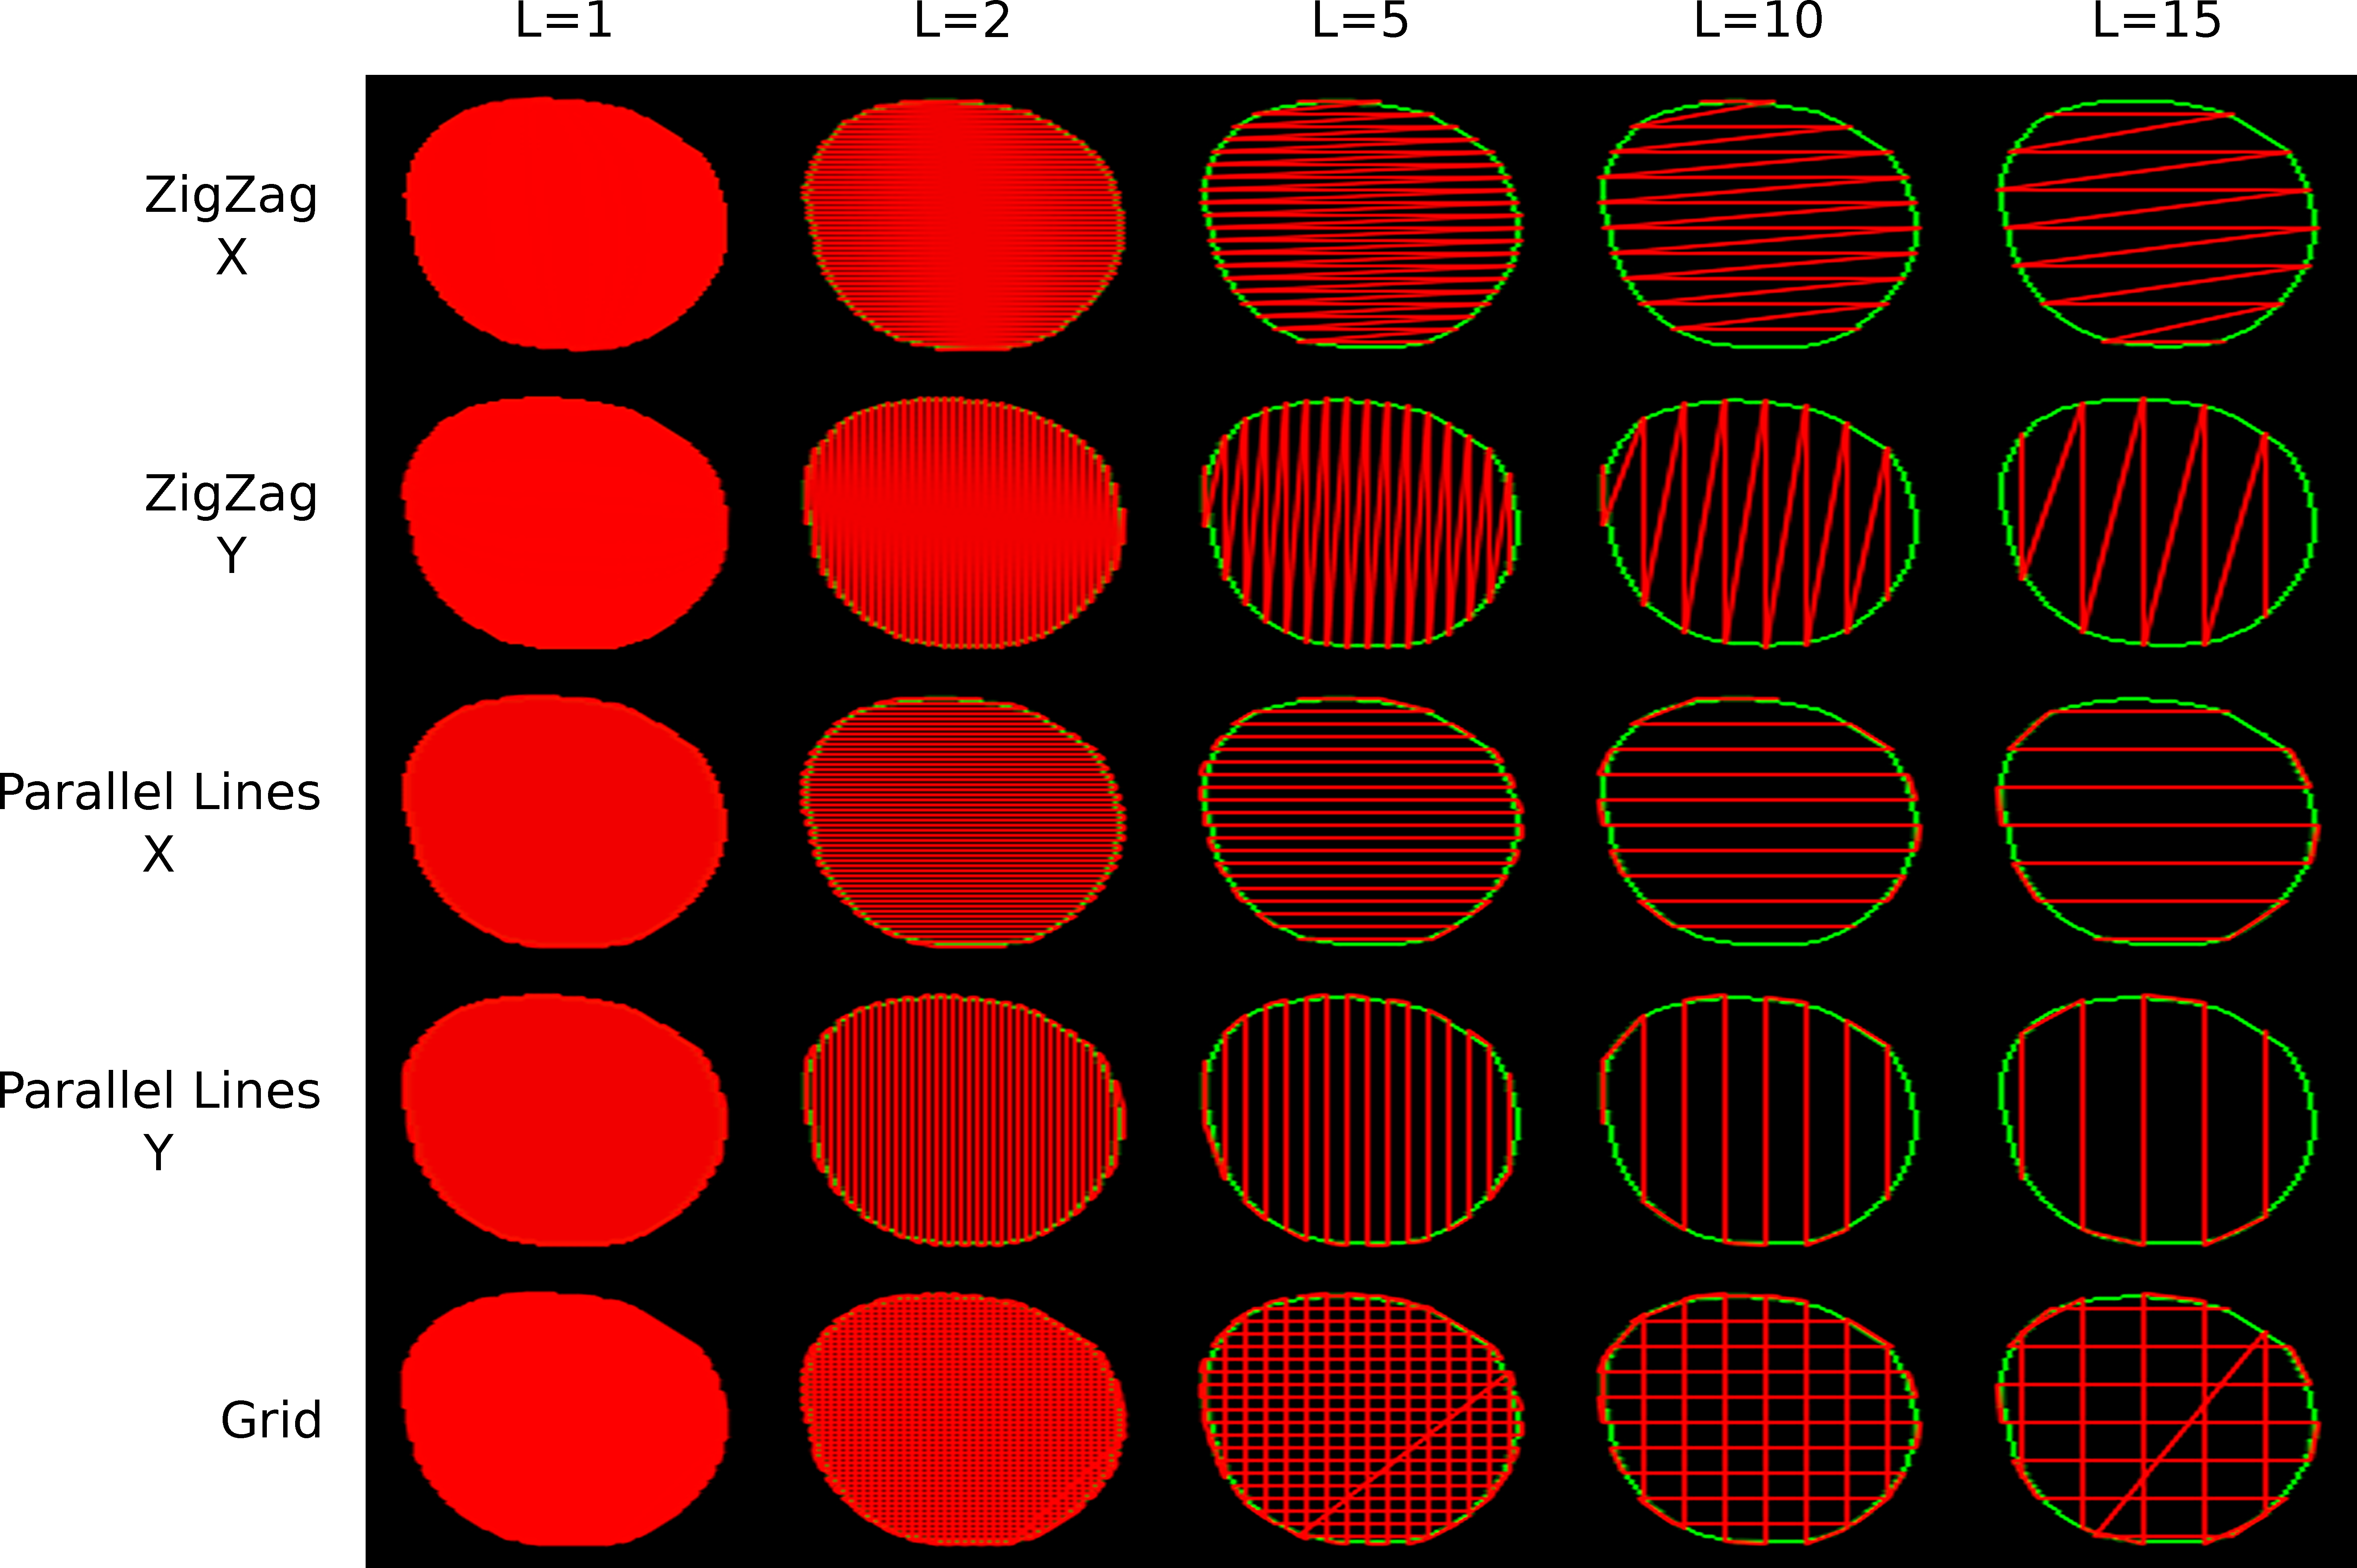
\includegraphics[width=.85\textwidth]{simulation_test_results_appendix_toolpath_wound_5}
	\caption{Path planning for wound model 5. The green line represents the segmented wound contour. The red line is the planned path. From left to right, the distance between lines, $L$, in pixels, is increasing. Smaller $L$ means more wound filling but also more bioink consumption. From top top bottom, the different paths are displayed. Each line corresponds to a different path planning strategy.}
	\label{fig:simulation_test_results_appendix_toolpath_wound_5}
\end{figure}

% section simulation_test_results_appendix_path_planning